\chapter{Discussion and future work}
\label{toc:discussion}
Everything is better when we stick together.
Side by side you and I are gonna win forever!
Lets party forever.
We're the same, I'm like you, you're like me---we're all working in harmony.

\section{Brainstorming}
We discuss the bigger picture of the thesis and further work jointly.
Main arguments:
\begin{enumerate}
    \item Formulating hierarchical models with strong constraints improves inference (See wind example). To expand on this, we need to improve our inference techniques as well~\parencite{ustyuzhaninov_compositional_2020}.
    \item It is often not clear what makes a hierarchical model good. Data association and wind showed that it goes beyond likelihoods, RL goes for interpretability. How do we formalize this? Interpretability is an important factor here!
    \item Going beyond regression, using models in pipelines or for specific tasks gives rise to performance measures. RL showed we can use it to test if a model behaves in a way we want it to behave. Going further, we can learn from probabilistic numerics to actually formalize what we want to see. For example, in BO~\parencite{bodin_modulating_2020} a surrogate maybe does not really have to be a good regressor. In RL, Bayesian inference over a policy might alow us to learn what actually matters in terms of a dynamics model (mountain car example)
\end{enumerate}

\section{Arguments}
Machine learning methods have seen great success recently in a wide range of digital domains such as speech recognition, computer vision or translation.
In such domains, data is abundant and the consequences of mistakes tend to be mild.
However, bridging the gap to applications in the physical world has proved challenging.
Problem domains like robotics, industrial control, decision support systems or the natural sciences introduce a new set of requirements.
ML-systems which operate in safety-critical areas, interact with people or carry responsibility must be robust, trustworthy and assessable.
As applications become more safety-relevant, gathering data through exploration can be problematic due to adverse consequences of failure.
Besides optimizing for good average-case performance, a responsible system needs to reason about plausible worst-cases and reliably avoid or inform about them.
ML-systems need to be verified by domain experts before deployment and are used to test hypotheses or make impactful decisions, emphasizing a need for interpretability.
Models are required to incorporate and reproduce expert knowledge and make consistent predictions.
A key technique that allows us to cope with these requirements are principled probabilistic models that allow us to explicitly represent and propagate uncertainties.
This allows us to both quantify confidence in predictions and take more unlikely but relevant scenarios into consideration.

At Siemens Research, I have worked on a number of pioneering applications of machine learning to industrial systems in safety-critical applications.
In industrial control problems, machine learning is often used to find more efficient or safer control strategies not obvious to the engineers designing a machine.
Relevant data for finding new strategies is scarce since the most valuable data such as when a machine will fail or how it will behave in new situations is never produced.
Finding exploration strategies is a collaborative task combining the knowledge of machine learning experts and domain experts.
Above all, interdisciplinary work requires a common language and understanding.
One of my research goals is to explore how to effectively formulate robust models together with domain experts to combine the available data with their knowledge.
This knowledge is often based on an intuitive understanding of the underlying physics leading to coarse expectations about system-behavior on different layers of abstraction.
In recent work\footnote{Bayesian Alignments of Warped Multi-Output Gaussian Processes, \url{https://arxiv.org/abs/1710.02766}}, we formulated a model that is capable of representing the complex interactions between turbines in a wind farm.
We combined strong hierarchical prior knowledge about wind propagation and turbine behavior with the flexibility of general function approximations to separate stochastic turbulence from adverse wake effects.
During my fellowship, I will build on this work and explore how abstract expert knowledge can be embedded in hierarchical models efficiently.

Machine learning models can be effective tools for communication with experts if they allow extensive inspection to achieve interpretability.
Besides allowing easier formulation of prior knowledge, interpretable models can be evaluated more extensively than black-box approaches.
Classical metrics such as low errors on test sets are often not enough for domain experts who are not machine learning specialists to build trust in a model.
Formulating principled generative models based on expert understanding allows us to reproduce their abstract expectations.
Combining such models with data allows us to gain new insights about the badly understood components of a system.
In recent work\footnote{Bayesian decomposition of multi-modal dynamical systems for reinforcement learning, \url{https://papers.mrksr.de/neurocomputing2020}}, we showed how a semantic decomposition of the dynamics of a reinforcement learning system significantly reduces the data requirements and produces interpretable solutions.
During my fellowship, I will generalize this work to explore how models can be evaluated by taking model components, generative samples and downstream tasks into account.

Many of the challenges faced in industrial applications of machine learning translate to applications in the natural sciences.
When applying machine learning in research contexts, care must be taken that models hold up to the requirements of scientific rigor.
When relying on models to understand new science, it is crucial to ensure their predictions are sensible and reliable.
Besides ensuring they do not hide complexity by making them interpretable, models need to be robust and reproducible.
Many black-box methods in use today depend on carefully tuned hyper-parameters to produce desired results, drawing their robustness into question.
Sound probabilistic model formulations make assumptions explicit and principled treatment of uncertainties makes models more robust to adverse effects.
In recent work\footnote{Data Association with Gaussian Processes, \url{https://arxiv.org/abs/1810.07158}}, we formulated a fully Bayesian interpretation of the data association problem.
One application of this method are noise separation tasks, where faulty sensor data can be separated into true readings and complex heteroscedastic noise while still producing informative uncertainties for downstream tasks.
I will continue this line of work to explore how model efficient formulations and approximations ensure applicability and robustness in practice.

I am passionate about making machine learning work in real world applications.
I plan to address the following research questions:
\begin{itemize}
    \item How do we formulate data-efficient models together with domain experts?
    \item How do we ensure models can be trusted to take responsibility?
    \item How do we implement models to yield robust results?
\end{itemize}
Successfully bridging the gap to to the physical world requires both advances in theory and interdisciplinary effort.
I want to explore how to effectively formulate structural and semantic priors which are both expressive and interpretable and extend our understanding of such priors.
I will build on my experience with formulating principled probabilistic models with domain experts in the natural sciences or the industry and identify promising research directions and collaborations.

I am interested in ways to evaluate models beyond error measures and marginal predictions, taking into account the shape of samples drawn from generative models or the behavior of different components of a hierarchy.
In recent work\footnote{Modulating Surrogates for Bayesian Optimization, \url{https://arxiv.org/abs/1906.11152}}, we presented a new interpretation of Bayesian optimization in which we formulate the surrogate to only model the components of the objective function that help in solving the optimization task.
I want to explore how downstream tasks can be taken into account in a principled manner in model design by formulating joint Bayesian models for learning pipelines.

Interpretable models and principled uncertainty propagation often require costly computations.
To implement models in practice, we need to rely on more efficient approximations.
In recent work\footnote{Compositional uncertainty in deep Gaussian processes, \url{https://arxiv.org/abs/1909.07698}}, we discussed shortcomings of current approximation to deep Gaussian process structures and how these shortcomings could be overcome.
I want to explore how the the benefits of principled statistical models can be combined with the efficiency of large parametric models to yield reliable and fast predictions in real world applications.

Our research projects have been successfully published in leading machine learning venues and are being deployed in industrial applications.
Our work on hierarchical GP models is being applied to challenging modeling tasks in the context of wind-turbines and gas turbines.
Principled uncertainty propagation allows us to derive controllers for gas turbines that improve power generation and reduce emissions.
Our work on Bayesian optimization is being used in large-scale automated design tasks.
Working on interdisciplinary projects in the industry has taught me to effectively collaborate in teams with diverse backgrounds and how to communicate machine learning to non-experts.
I have gained experience in identifying promising applications of machine learning, developing concepts together with domain experts, efficient experimentation and implementation and deployment of models to embedded devices.

During my research, I have actively sought to bring industrial and academic experts together.
I have established collaborations with academic institutions, initiated a three-month research stay of an academic advisor at Siemens and designed and organized an international workshop on uncertainty propagation with 25 attendees from academia and the industry.
During my fellowship, I want to continue establishing collaborations both in academia and with industrial partners.
I am convinced that taking the step to the physical world is one of the most important challenges for machine learning today, requiring models with principled statistical foundation and broad interdisciplinary collaboration.
I think I am well suited to tackle these challenges as I have worked on relevant applications, experience in interdisciplinary groups and the required theoretical background.


\section{Inference in hierarchical models}
\begin{figure}[t]
    \centering
    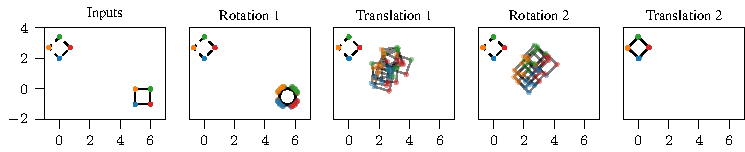
\includegraphics[width=\textwidth]{rotated_squares_example}
    \caption{
        \label{fig:rotated_squares_example}
        Compositional model (toy example): the transformation of the solid rectangle onto the dashed one is decomposed as $T_2 \circ R_2 \circ T_1 \circ R_1$ where $R_i$ and $T_i$ are rotations and translations. Different sampled realizations of these transformations are overlaid, showing the \emph{compositional uncertainty}. Approximating $R_i$ and $T_i$ as independent transformations does not allow us to capture such uncertainty, collapsing to a single realisation of the composition.
    }
\end{figure}


\section{Bayesian Optimization}
\begin{figure}[t]
    \centering
    \raisebox{-0.5\height}{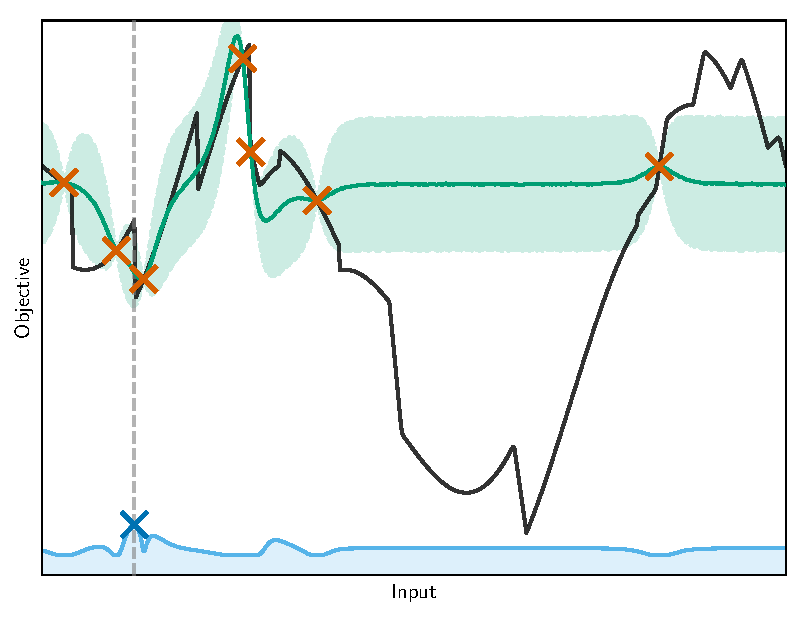
\includegraphics[trim=15 15 0 0, clip, width=0.25\textwidth]{robust_bo_erik/illustrative_figure/gp.pdf}}
    \raisebox{-0.5\height}{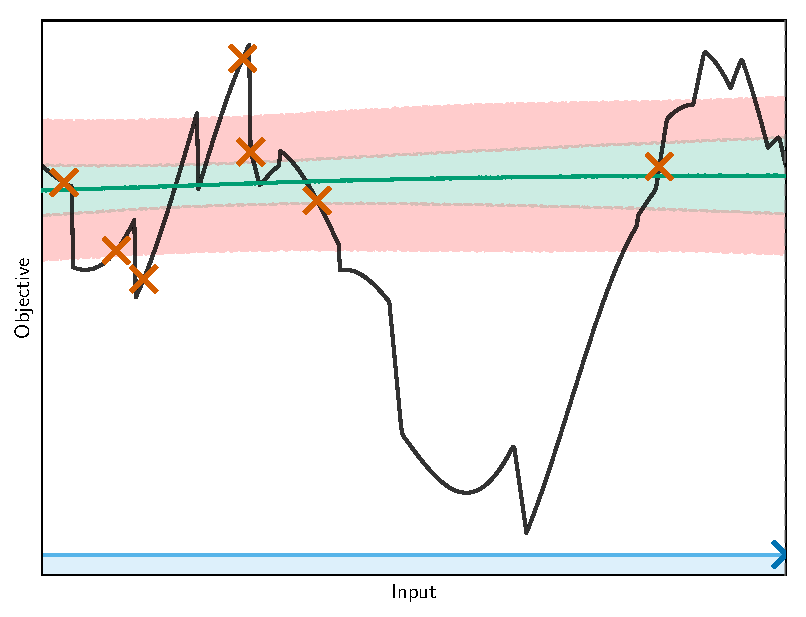
\includegraphics[trim=15 15 0 0, clip, width=0.25\textwidth]{robust_bo_erik/illustrative_figure/homo_gp.pdf}}
    \raisebox{-0.5\height}{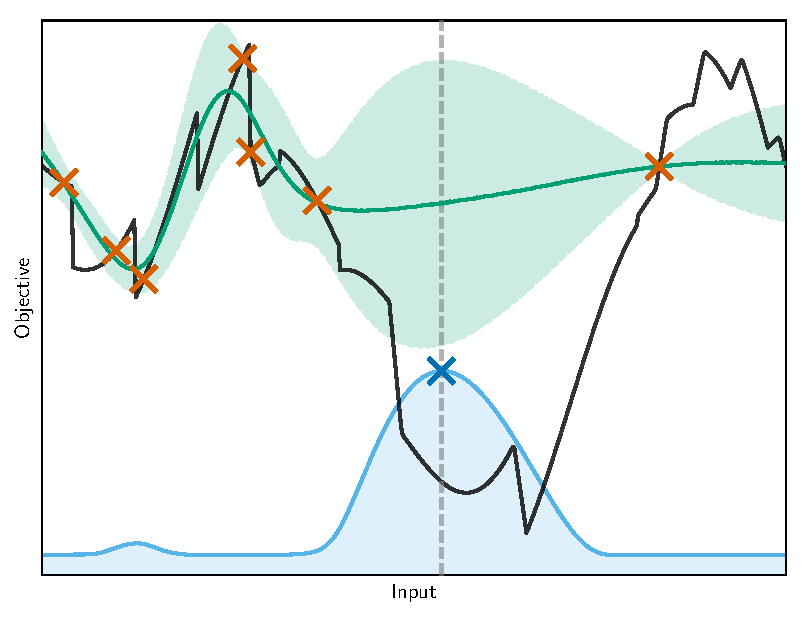
\includegraphics[trim=15 15 0 0, clip, width=0.25\textwidth]{robust_bo_erik/illustrative_figure/modulating_lgp.pdf}}
    \raisebox{-0.45\height}{{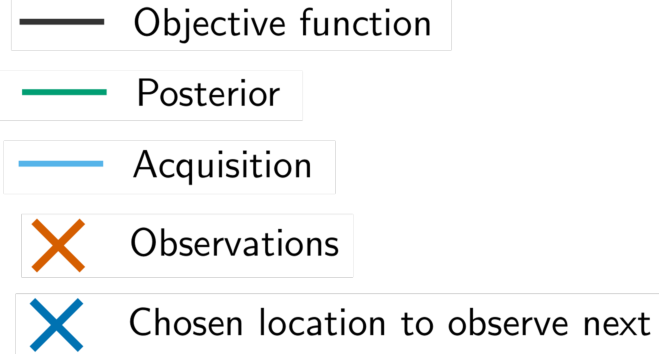
\includegraphics[width=0.20\textwidth]{robust_bo_erik/illustrative_figure/legend_compact.pdf}}}
    \caption{
        \label{fig:bo:posterior}
        As a result, the acquisition function can utilize a confidently discovered global trend to increase the efficiency of the search.
    }
\end{figure}


\section{Reinforcement Learning}
\begin{figure}[t]
    \centering
    \includestandalone{mountaincar_system}
    \caption{
        \label{fig:mountaincar:system}
        Mountaincar system
    }
\end{figure}
\begin{figure}[t]
    \centering
    \includestandalone{graphical_model_rl_deep_gp}
    \caption{
        \label{fig:mountaincar:graphical_model}
        Deep GP RL graphical model.
    }
\end{figure}
\begin{figure}[tp]
    \centering
    \includestandalone{mountaincar_policy_01}
    \includestandalone{mountaincar_policy_10}
    \includestandalone{mountaincar_policy_25}
    \caption{
        \label{fig:mountaincar:policy}
        Mountaincar policies after different iteration counts.
    }
\end{figure}
